\begin{center}
\footnotesize\noindent\fbox{
	\parbox{\textwidth}{
	Utilizzare le function degli Esercizi 4.1 e 4.6 per graficare l'approssimazione della funzione di Runge sull'intervallo \([-6, 6]\), per \(n = 2, 4, 6, \ldots, 40\). \\ \\Stimare numericamente l'errore commesso in funzione del grado \textit{n} del polinomio interpolante.
	}
}\end{center}

\noindent Di seguito i grafici che mostrano i polinomi interpolanti di grado \textit{n} calcolati usando come punti di interpolazione quelli corrispondenti alle \textit{n} ascisse di Chebyshev. \\

\noindent\small\begin{tabular}{l*{5}{c}}
\hspace{3.5cm}\(n=2\) & \(n=4\) \\
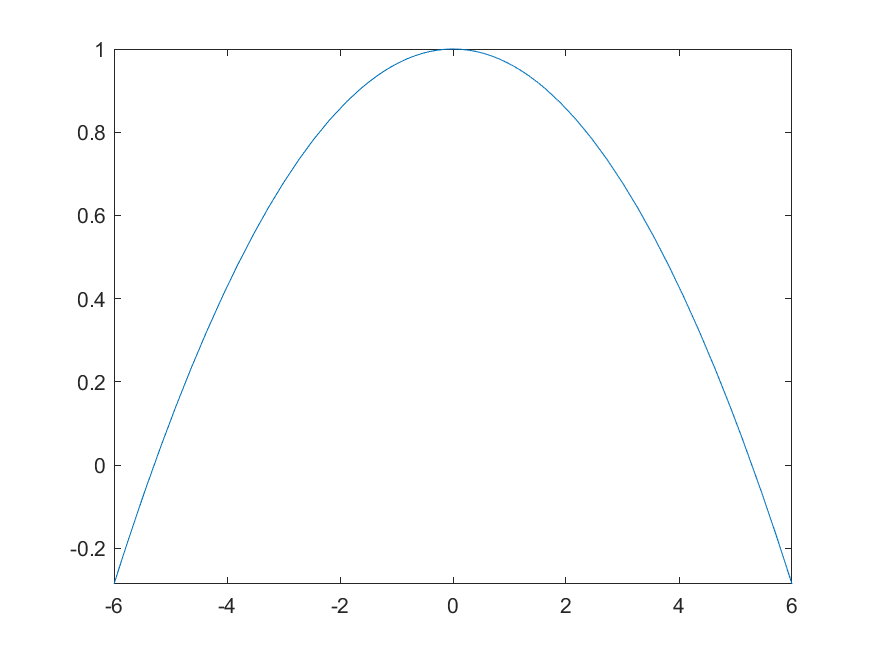
\includegraphics[scale=0.5]{cap4/4_7/2.png} &  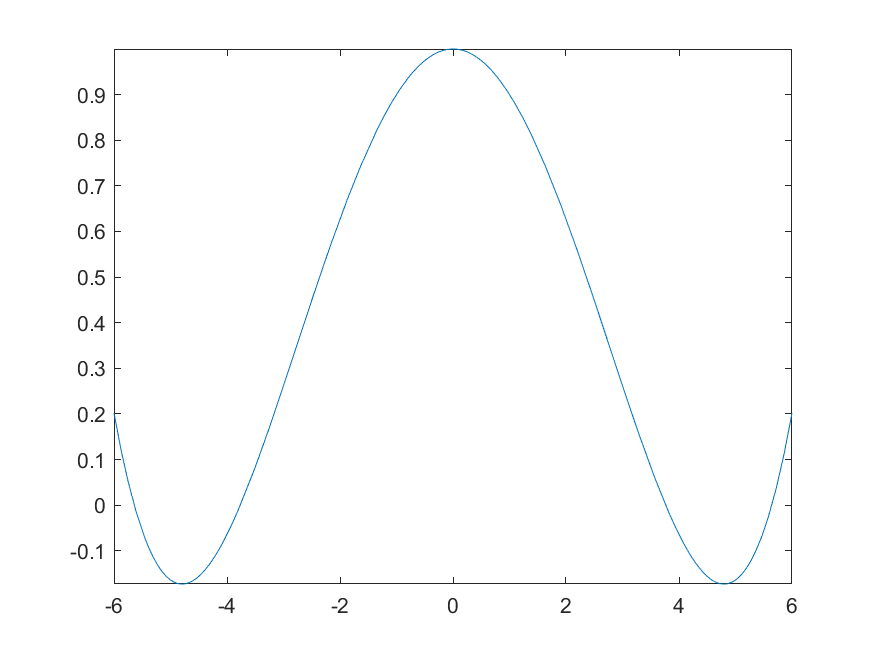
\includegraphics[scale=0.5]{cap4/4_7/4.png} \\

\hspace{3.5cm}\(n=6\)& \(n=8\) \\
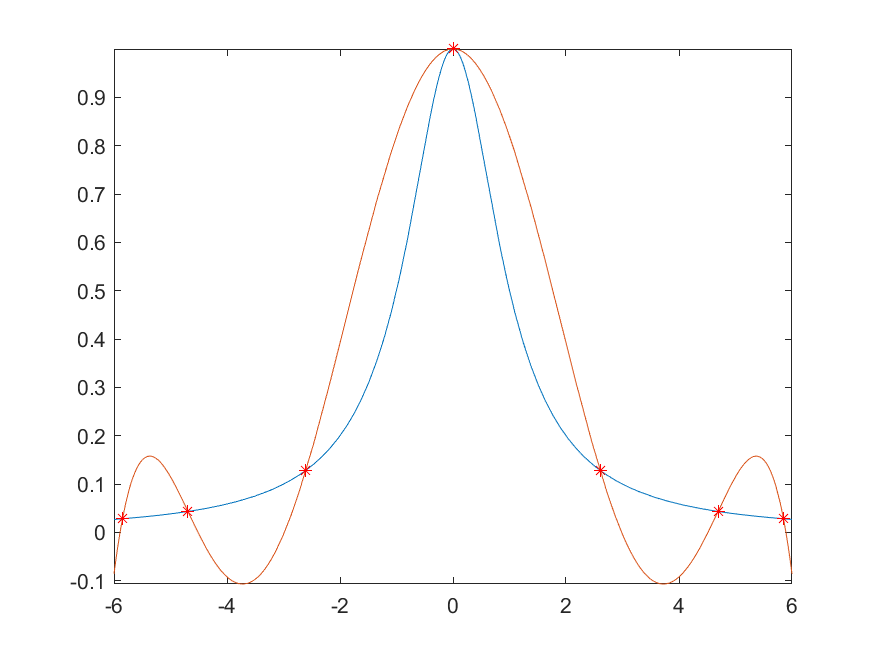
\includegraphics[scale=0.5]{cap4/4_7/6.png} &  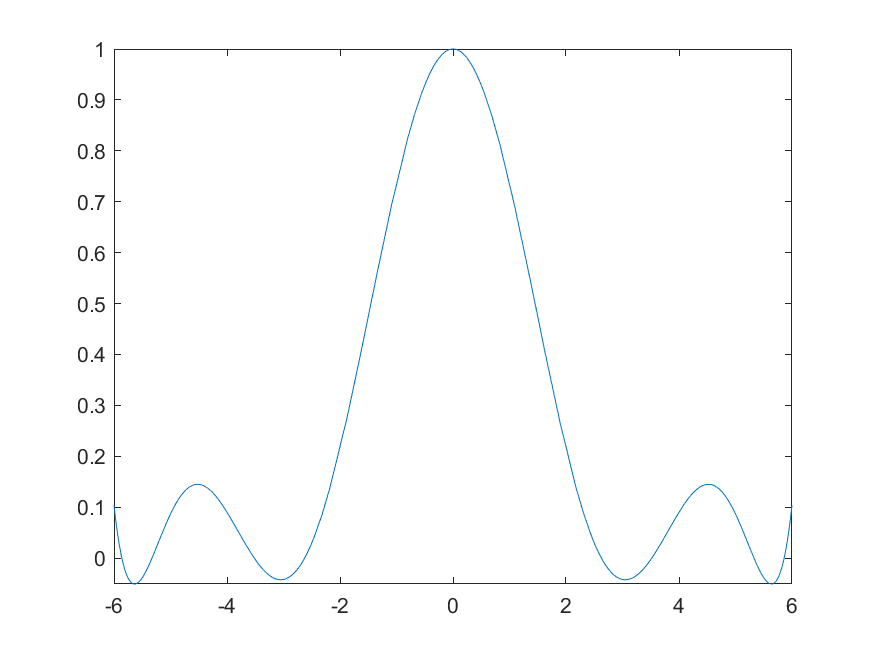
\includegraphics[scale=0.5]{cap4/4_7/8.png} \\

\hspace{3.5cm}\(n=10\) &  \(n=12\) \\
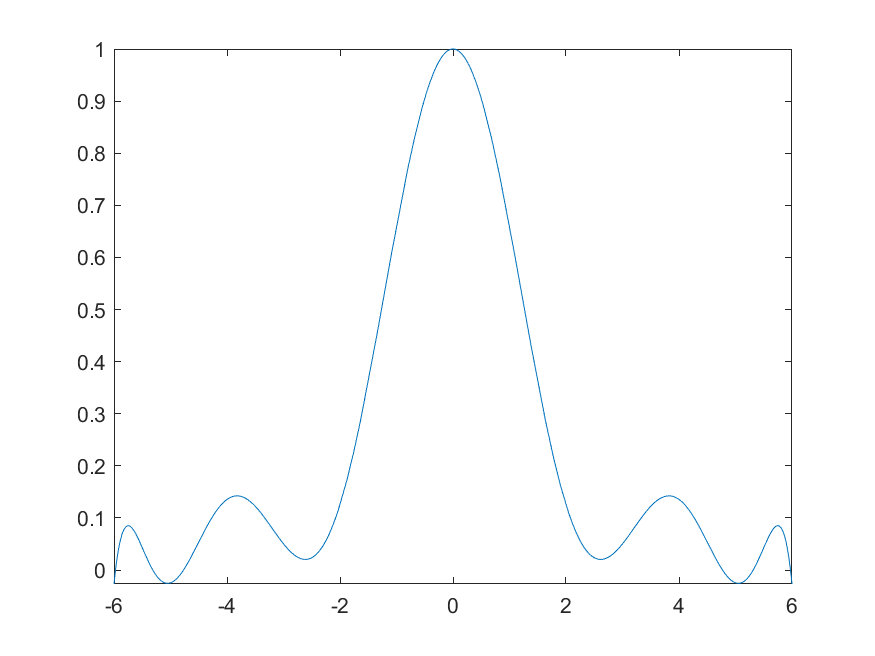
\includegraphics[scale=0.5]{cap4/4_7/10.png} &  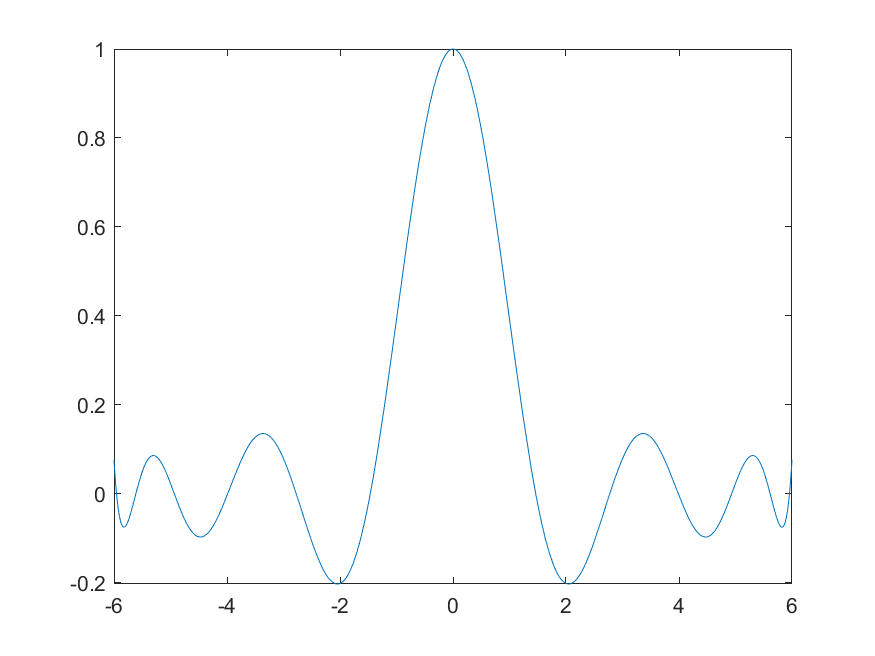
\includegraphics[scale=0.5]{cap4/4_7/12.png} \\
\end{tabular} \\ \\

\small\begin{tabular}{l*{5}{c}}
\hspace{3.5cm}\(n=14\) &  \(n=16\) \\
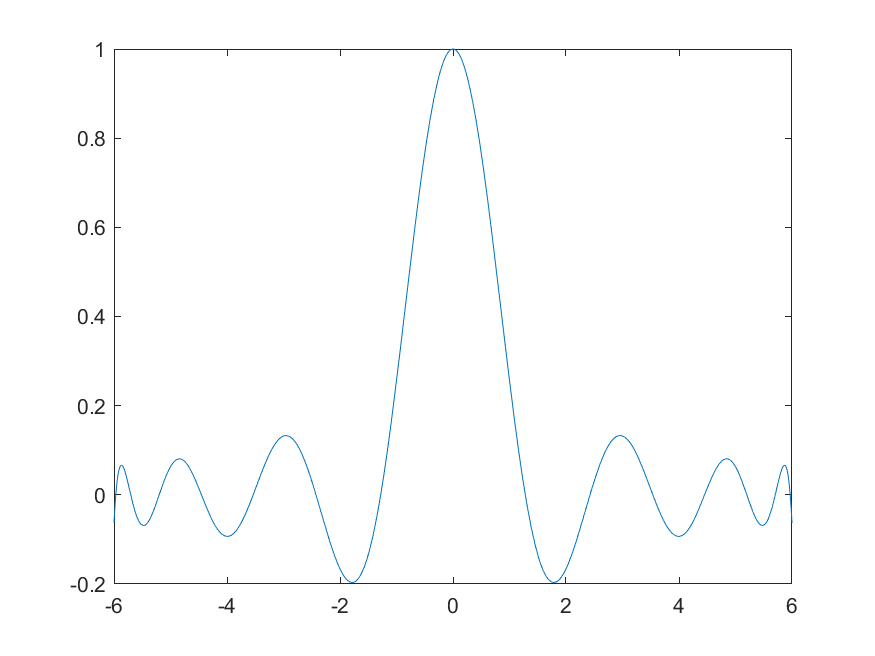
\includegraphics[scale=0.5]{cap4/4_7/14.png} &  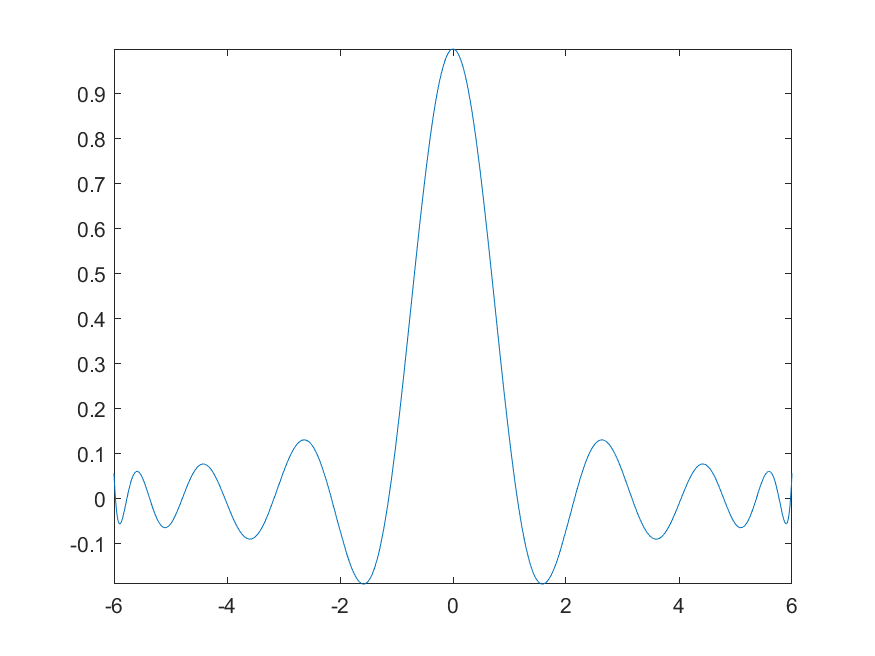
\includegraphics[scale=0.5]{cap4/4_7/16.png} \\

\hspace{3.5cm}\(n=18\) &  \(n=20\) \\
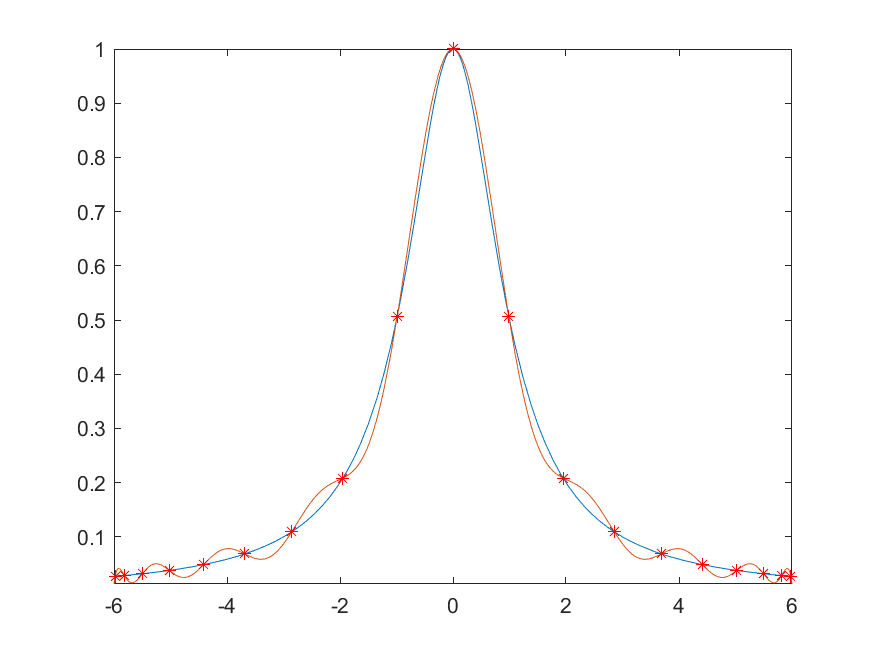
\includegraphics[scale=0.5]{cap4/4_7/18.png} &  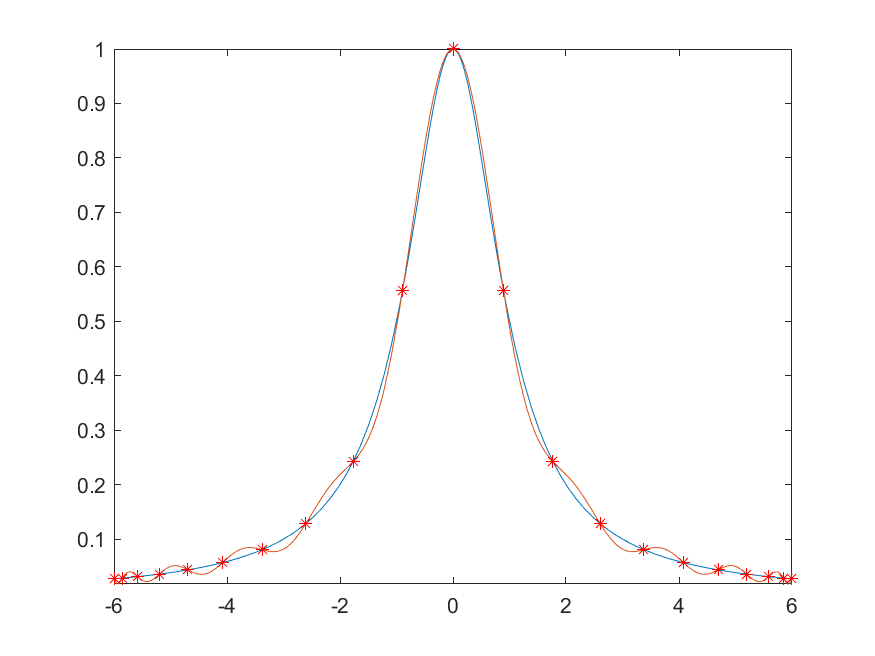
\includegraphics[scale=0.5]{cap4/4_7/20.png} \\

\hspace{3.5cm}\(n=22\) &  \(n=24\) \\
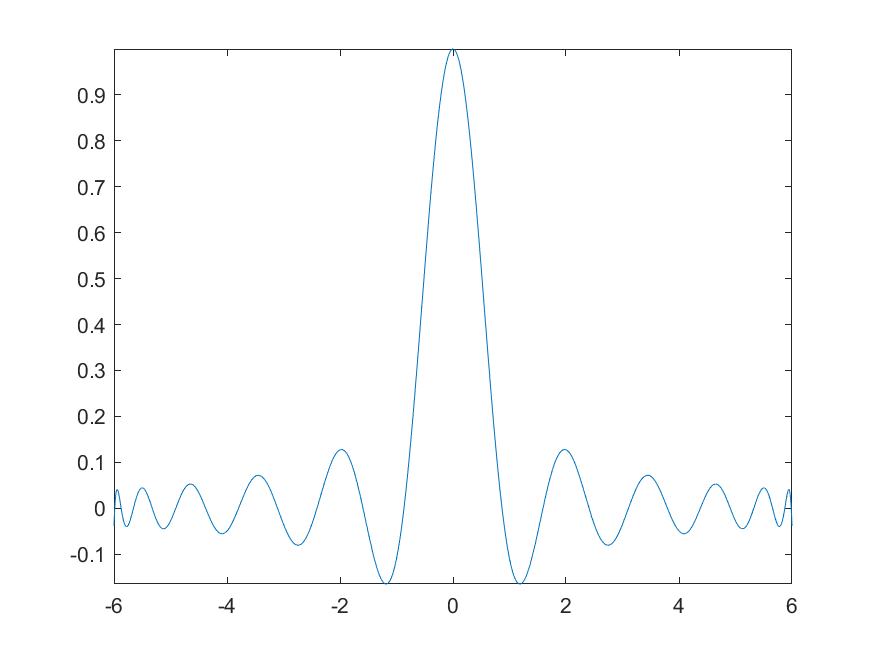
\includegraphics[scale=0.5]{cap4/4_7/22.png} &  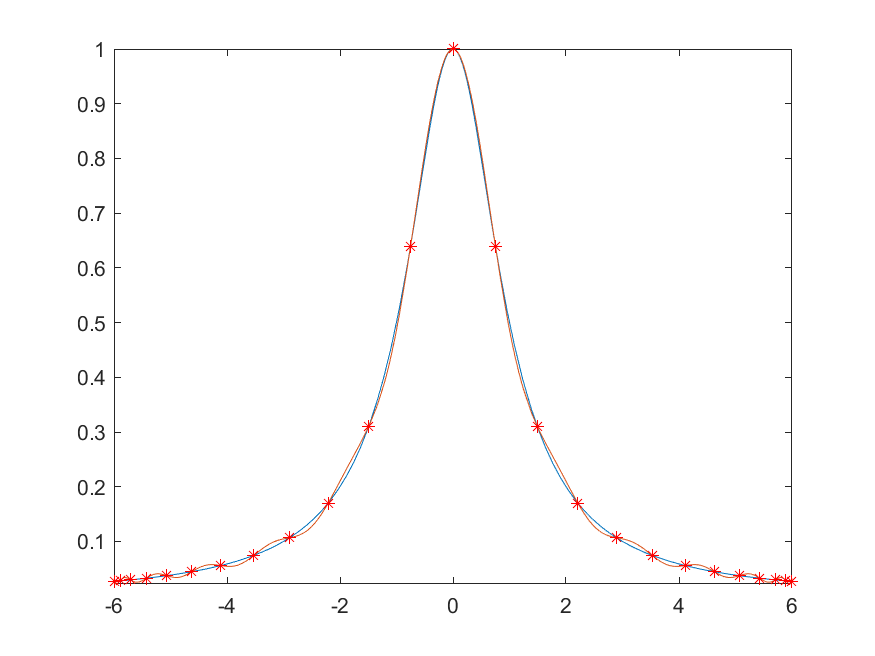
\includegraphics[scale=0.5]{cap4/4_7/24.png} \\

\hspace{3.5cm}\(n=26\) &  \(n=28\) \\
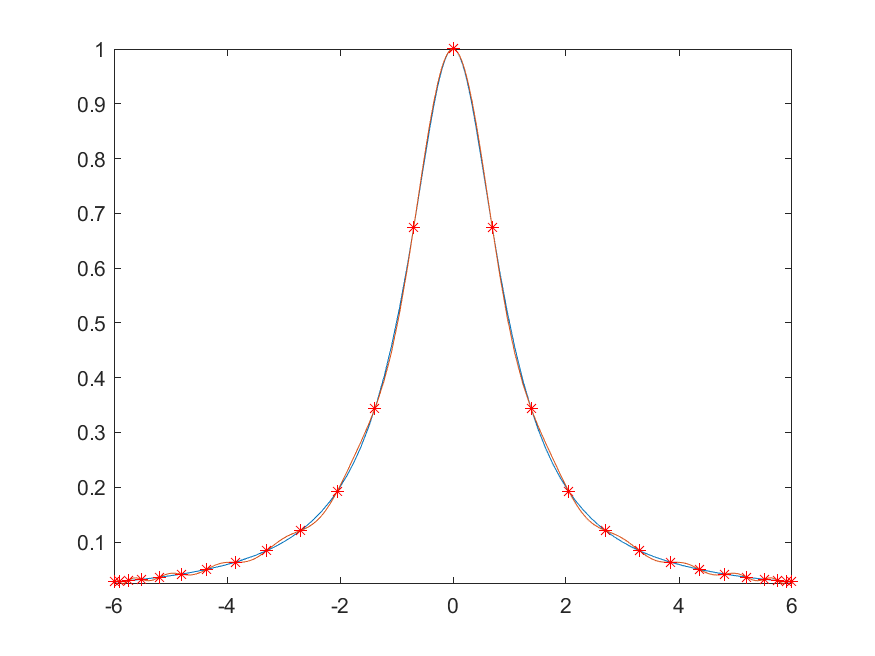
\includegraphics[scale=0.5]{cap4/4_7/26.png} &  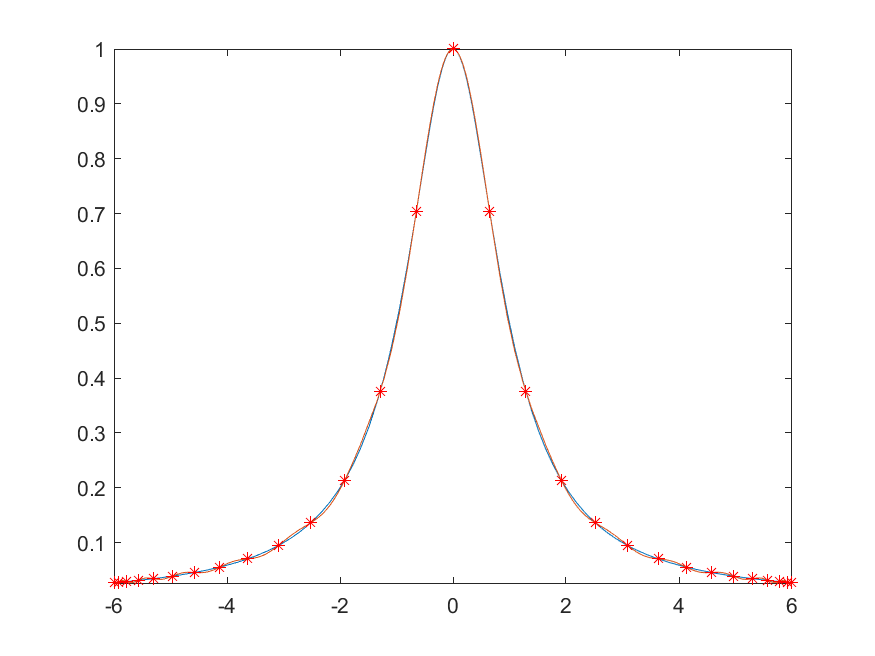
\includegraphics[scale=0.5]{cap4/4_7/28.png} \\
\end{tabular}

\small\begin{tabular}{l*{5}{c}}
\hspace{3.5cm}\(n=30\) &  \(n=32\) \\
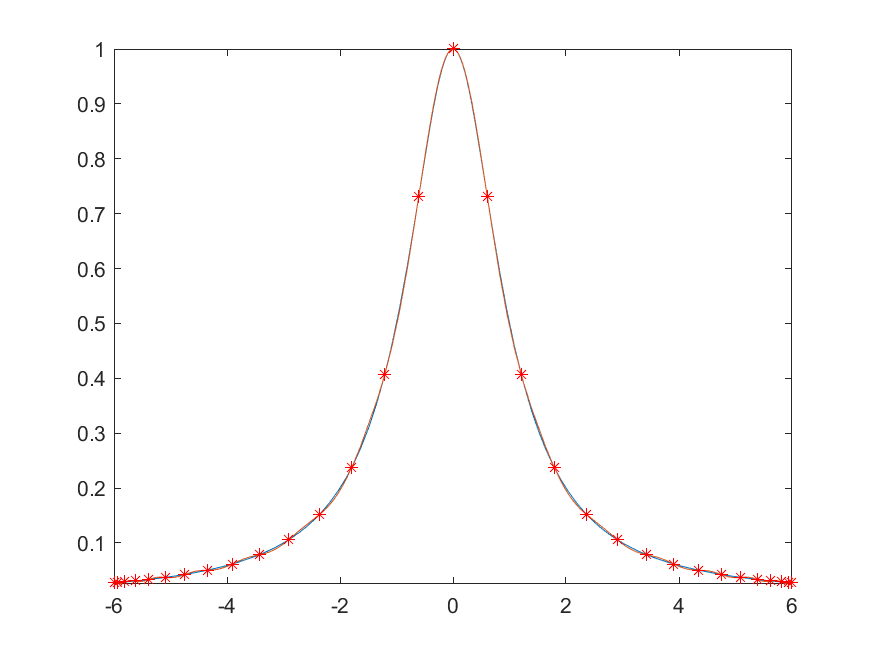
\includegraphics[scale=0.5]{cap4/4_7/30.png} &  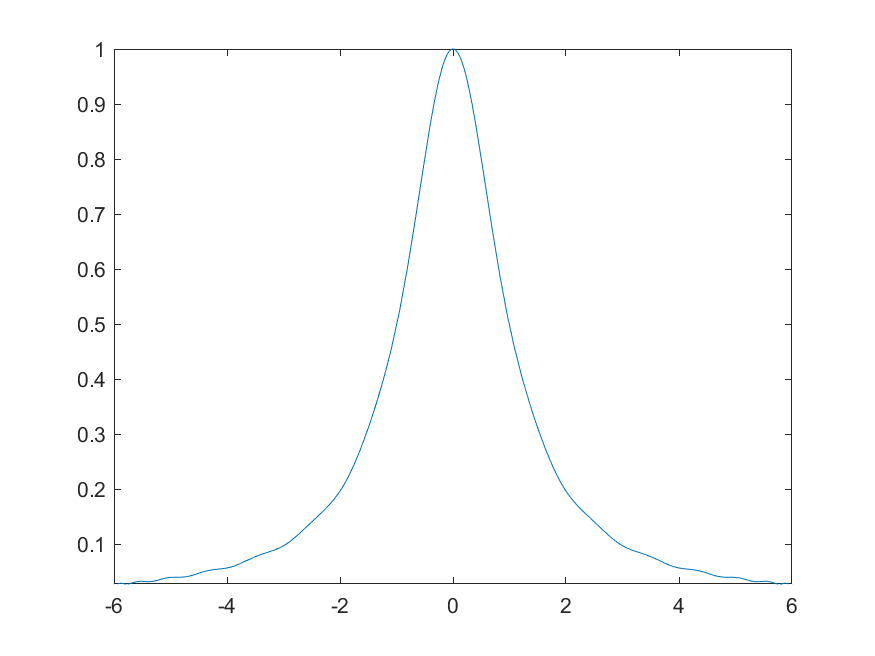
\includegraphics[scale=0.5]{cap4/4_7/32.png} \\

\hspace{3.5cm}\(n=34\) &  \(n=36\) \\
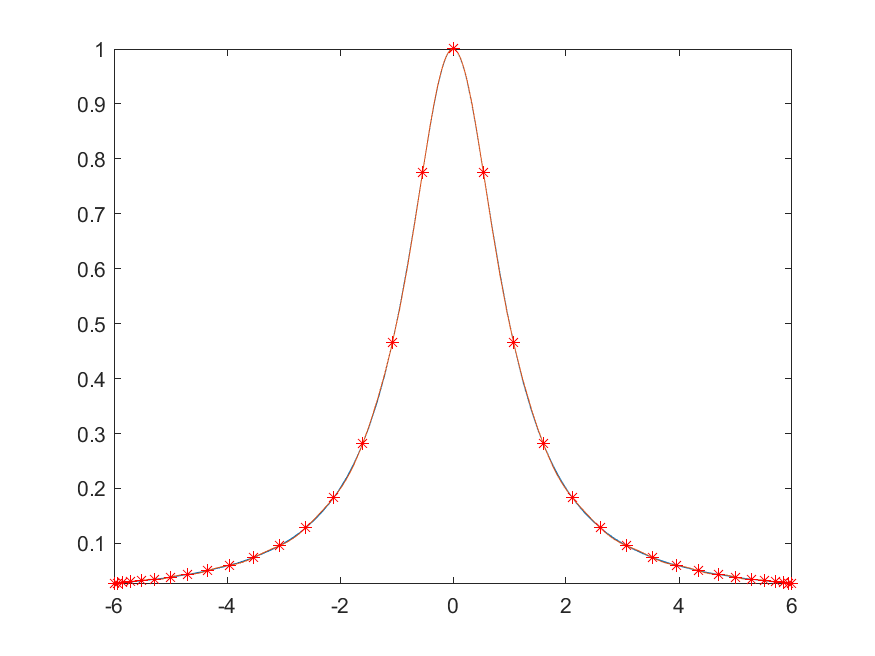
\includegraphics[scale=0.5]{cap4/4_7/34.png} &  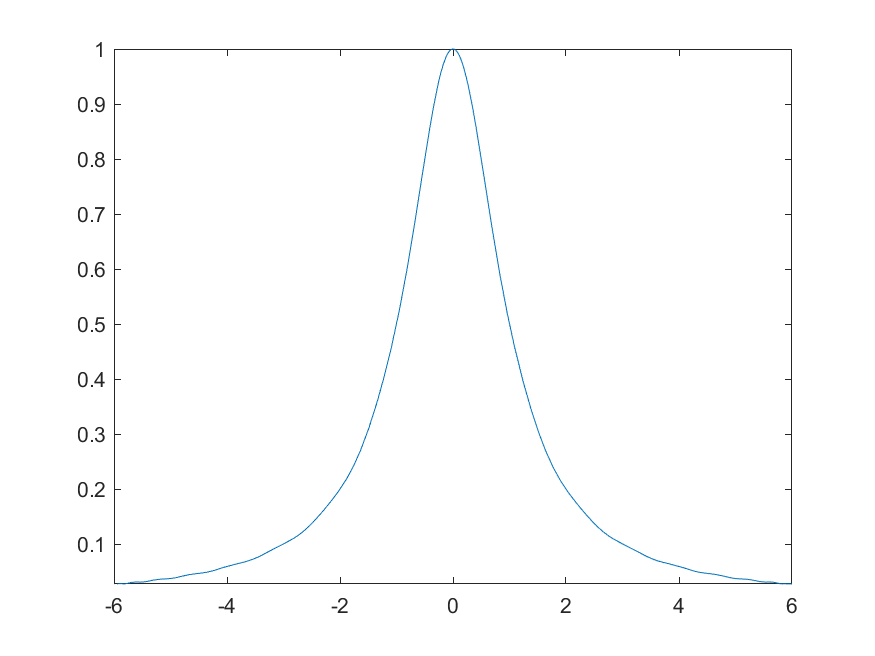
\includegraphics[scale=0.5]{cap4/4_7/36.png} \\

\hspace{3.5cm}\(n=38\) &  \(n=40\) \\
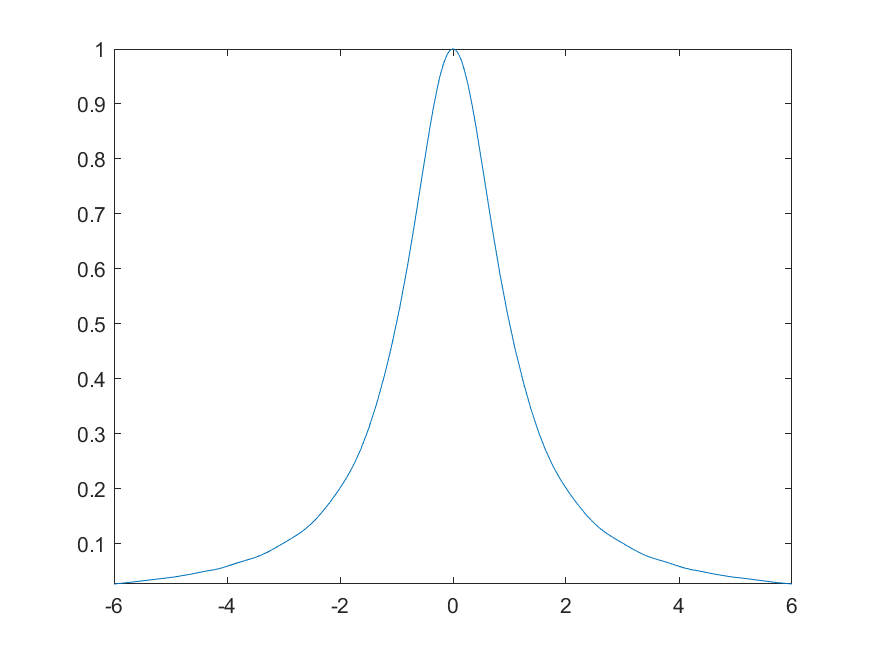
\includegraphics[scale=0.5]{cap4/4_7/38.png} &  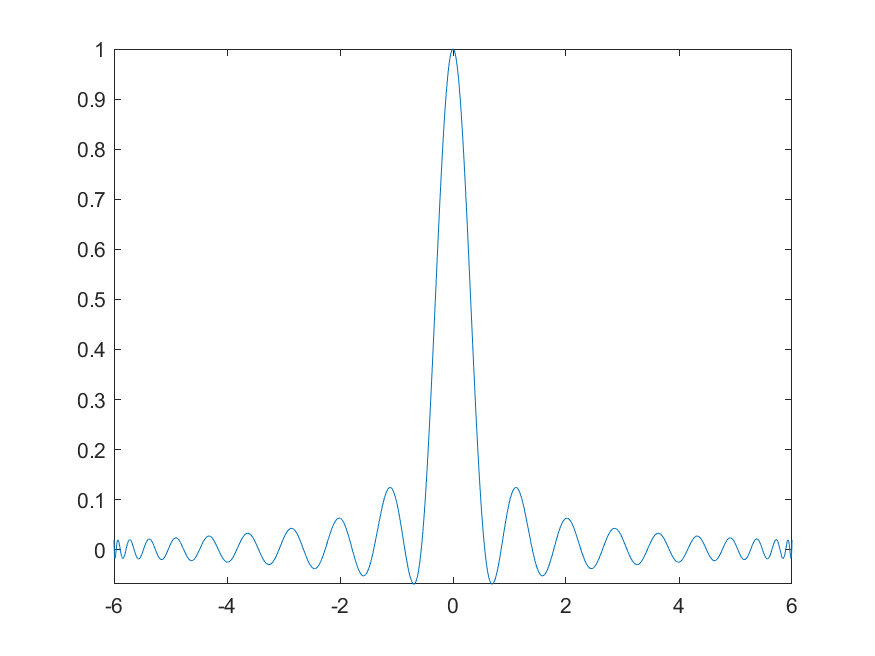
\includegraphics[scale=0.5]{cap4/4_7/40.png} \\
\end{tabular}

\begin{center}
\scriptsize{\(r(x) = \frac{1}{1+25x^2}\):}\\
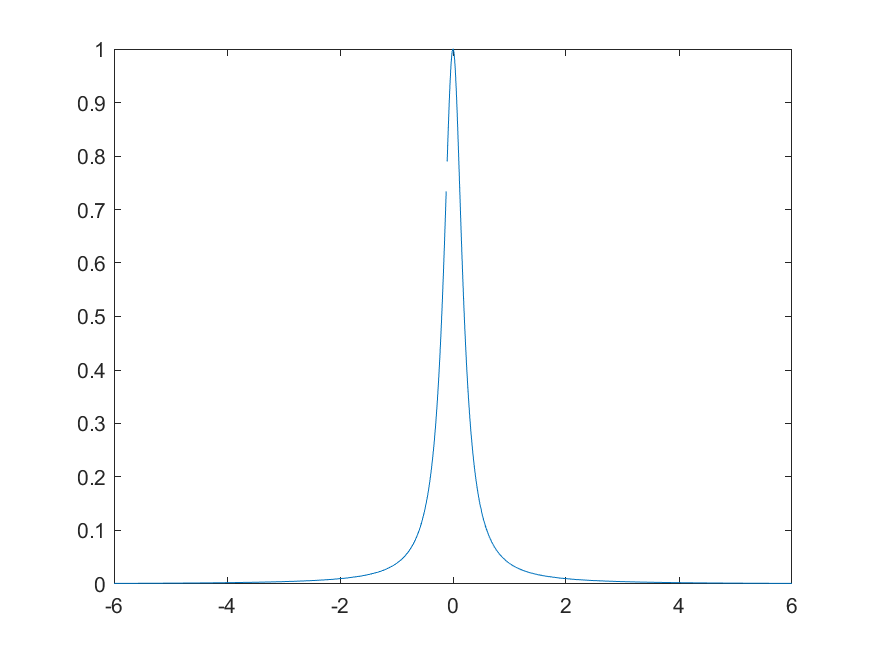
\includegraphics[scale=0.45]{cap4/4_7/runge.png}
\end{center}


\noindent Riguardo alla stima dell'errore commesso, ricordando che, grazie alla scelta dei nodi di Chebyshev come punti di interpolazione, per funzioni sufficientemente regolari abbiamo:
\[
||e|| = \frac{||f^{(n+1)}||}{(n+1)!2^n}
\]

\noindent Sono quindi state calcolate le seguenti stime:

\begin{center}
	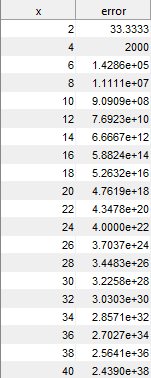
\includegraphics[scale=0.5]{cap4/4_7/4_7_error.png}
\end{center}

\noindent Come si pu\'o facilmente vedere, quello che avviene \'e ??? coi nodi di cheby dovrebbe abassare l'errore...

CONTROLLARE IL CONTO DELL ERRORE E A STO PUNTO RIFARE ANCHE I GRAFICHETTI DEL CAZZO

\noindent Il codice Matlab con cui sono stati realizzati i grafci e la tabella mostrati sopra \'e il seguente:

\lstinputlisting[language=Matlab]{cap4/4_7.m}
